\documentclass[11pt]{article}

\usepackage[utf8]{inputenc}
%%\usepackage[T1]{fontenc}
\usepackage{graphicx}
\usepackage[linktocpage=true]{hyperref}

%%Page layout
\usepackage[margin=2.0cm]{geometry}
\usepackage{bookmark}

%%Figures
\usepackage{float}

\usepackage{mathpazo}

%%Font and Numbers
\renewcommand*\rmdefault{dayrom}
\usepackage[T1]{fontenc}
\normalfont
\usepackage{enumitem}

%%Packages for Referrences
\usepackage{url}
\usepackage{etoolbox}
\patchcmd{\thebibliography}{\section*{\refname}}{}{}{}
\patchcmd{\thebibliography}{\addcontentsline{toc}{section}{\refname}}{}{}{}

%%Group Comments
\usepackage{verbatim}

\begin{document}
\renewcommand{\familydefault}{\sfdefault}
\begin{titlepage}
	\newcommand{\HRule}{\rule{\linewidth}{0.5mm}}
	\begin{center}
		            
		\textsc{\LARGE Alabama Liquid Snake}\\[0.8cm]
		\textsc{\Large University of Pretoria}\\[0.5cm]
		\textsc{\large Epi-Use}\\[0.5cm]
		    
		\HRule\\[0.4cm]
		    	
		{\huge\bfseries Botic - Privacy aware chatbot}\\[0.2cm]
		    	
		{\huge System Architectural Design}\\[0.2cm]
		
		\HRule\\[0.5cm]
		
		\textsc{Justin Grenfell} - u16028440 \\[0cm]
		\textsc{Peter Msimanga} - u13042352 \\[0cm]
		\textsc{Alicia Mulder} - u14283124 \\[0cm]
		\textsc{Kyle Gaunt} - u15330967 \\[0cm]
		\textsc{Lesego Mabe} - u15055214 \\[0cm]
		    
	\end{center}
\end{titlepage}
\tableofcontents
\newpage
\section{Architectural Design}

\subsection{Determine System Types}
%This ought to be done in layers i.e. first layer of granularity

From a top view of the entire system, we have observed that the system is more of an interactive system type. Our system is focused on the customer's interaction with the Chatbot, the customer support's interaction, and the administrator's interaction. This means that the interaction begins and ends with each user. The results in the ordering of all subsystems into a number of layers. This has the consequence of creating a clear and well-documented separation of concerns\cite{Book:2}. 

The layers that result are the following:
\begin{enumerate}
	\item The User Interface Layer
	\item The Chatbot Layer
	\item The Training Layer
	\item The Persistance Layer
\end{enumerate}
*This comes from the application of a 4-Tier Architecture.

These four layers we treat as the total system's four main subsystems. Each of these layers, or subsystems, produce exhibit system types of their own. Going into each, we will apply the architectural design process until the we find that the individual leaf node elements are relatively easy to design and implement\cite{Book:1}. \\*

Now we have a look at the "User Interface Layer." This layer deals heavily with actor requests and responses; all actors primarily interact with this subsystem in order satisfy business processes. This is clearly an interactive subsystem.\par

Looking at the Chatbot layer, we observe that the layers in a transformational subsystem. The Support layer, or rather the Training layer we observe a transformational subsystem. The Perisistance Layer, however, is very clearly an object-persistence subsystem.

\subsection{Architectural Tactics}

In order to achieve and adhere to our quality attributes, we use architectural tactics. These are design decisions that influence the achievement of a quality attribute as they directly affect the system's response to some stimulus\cite{Book:2}.

Below we list the architectural tactics that will be used satisfy our system's quality attributes (non-functional requirements), by order of the nonfunctional requirements listed above:

\subsubsection{Availability}
In order to fascilitate the application of tactics that improve availability, we would have to include the following into our system:
\begin{itemize}
	\item[] 1. Logging of faults
	\item[] 2. Notifying appropriate entities of the faults
	\item[] 3. Disable the source of events causing the fault
	\item[] 4. Be temporarily available if need be
	\item[] 5. Fix or mask the fault/failure
	\item[] 6. or Operate in a degraded mode
\end{itemize}

In order for these to be effected, faults need to be detected, the system needs to be able to recover from faults, and it is appropriate to have a measure of preventing faults before they happen.\\*

In order to log faults, the fault detection mechanism or tactic need to be able to store the detected 'faulty' state. The memento design pattern would clearly be useful here. We can even go as far as to have types of faults being associated with the types of mechanisms set out to identify each. For these, we may apply the Abstract Factory Pattern in order to produce specific fault logs, and store them in our fault logging database through the memento pattern. Event's can be stored in this way, so that we may be able to have a trace of operations that led to an error.\\*

Once that is stored in the caretaker, which in and of itself is a state change, we notify the module responsible for notifying the relevant parties of faults in the system. In order to effect these responsibilities, we would have to assign functionality that stores fault logs, and notifies users. These will be done in reference to use cases, because availability is an attribute that affects users - which are the actors in the use cases. The fault detection mechanisms (architectural tactics) depend on the particular operations of the modules, thus each of the modules or subsystems stand to have their own fault detection mechanisms (availability architectural patterns). This logic applies to tactics responsible for recovering from faults, and preventing faults.\\*

The table below provides the subsystems yeilded from functional clusters for high cohesion, and their system types as well as our chosen fault detection tactic, recovery tactic and fault prevention tactic. These are only subsystems that are necessary, and ordered according to priority. The architectural tactics are solution specific, therefore we expect to add many more of them as the development of the project continues; software engineering is a wicked problem afterall:

\begin{center}
	\hspace*{-1.2cm}\begin{tabular}{|c|c|c|c|c|}
		\hline
		Subsystem & Subsystem Type & Fault Detection & Recovery from Faults & Fault Prevention \\
		\hline
		Chatbot Subsystem & Transformational Subsystem & ping/echo, Retry & Exception Handling & Removal from Service\\
		\hline
	\end{tabular}	
\end{center}
Please note that the Chatbot Subsystem consists of the Message Scraper, Classifier and the Response Generator subsystems; thus all the mentioned tactics actually apply to each of this subsystem's components.

Two modules will be produced here: one for log management, and another for notification. These require that data be persisted.

\subsubsection{Security}
Looking at the quality requirements involving security in following the design checklist specified by \cite{Book:1}, we find that it is useful to use physical security as a model for software security as indicated by \cite{Book:2}. This results in the four categories of focus for this quality attribute: detect, resist, react, and recover. \\*

In order to support the design and the analysis of security in our system we will pay attention to the following, and ensure that these responsibilities are assigned and met:
\begin{itemize}
	\item[] 1. Identify the actor
	\item[] 2. Authenticate the actor
	\item[] 3. Authorize actors
	\item[] 4. Grant or deny access to data or services
	\item[] 5. Record attempts to access or modify data or services
	\item[] 6. Encrypt data
	\item[] 7. Recognize reduced availability for resources or services and inform appropriate personnel and restrict access
	\item[] 8. Recover from an attack
	\item[] 9. Verify checksums and hash values
\end{itemize}
 With regards to our data we shall ensure that the following is observed:
\begin{itemize}
	\item[] 1. Seperation of data of different sensitivities
	\item[] 2. Ensure different access to data of different sensitivities
	\item[] 3. Ensure that access to sensitive data is logged and that the log files is suitably protected
	\item[] 4. Ensure that data is suitably encrypted and that keys are separated from the encrypted data
	\item[] 5. Ensure that data can be restored if it is inappropriately modified
\end{itemize}

This attribute modifies or enhances modules introduced in the availability requirement analysis above, this includes the assignment of new responsibilities in particular, certain logs have to be stored securely-- those logging access to sensitive information. It also makes use of the notification module to let the appropriate personnel know that their system is being attacked, when these attacks are detected.\\*

The table below includes the architectural tactics we will employ with respect to each of the four categories (detection, resistance, reaction, and recovery) we defined earlier, the subsystems and their subsystem types. These are in order of priority:
\begin{center}
	\hspace*{-1.5cm}\begin{tabular}{|p{3cm}|p{3cm}|p{3cm}|p{3cm}|p{3cm}|p{3cm}|}
		\hline
		Subsystem & Subsystem Type & Detection & Resistance & Reaction & Recovery \\
		\hline
		User Interface Subsystem & Interactive Subsystem & Detect service denial, Detect message delay & Identify actors, Authenticate actors, Authorize actors, Encrypt data, Separate entities & Revoke access, Lock computer, Inform Actors & Maintain Audit Trail \\
		\hline
		Chabtot Subsystem & Transformational Subsystem & Verify Message Integrity, Detect service denial & Identify actors, Authorize actors, Encrypt data & Revoke access, Inform Actors & Maintain Audit Trail \\
		\hline
		Chatbot Trainer Subsystem & Transformational Subsystem & & Authorize actors, Encrypt data & Inform Actors & Maintain Audit Trail, Data Model checklist above* \\
		\hline
		Database Subsystem & Database subsystem & & Authorize actors, Encrypt data, Separate entities & Inform Actors & Maintain Audit Trail, Data Model checklist above* \\
		\hline
	\end{tabular}
\end{center}
Note: we mention the UI subsystem, but what we really mean are the operations performable by the roles of Administrator and Customer Representative. The UI is how they interact with the system.

These are not meant to be exhaustive; they are meant to be revised according to future needs and adapted with feedback.

\subsubsection{Reliability}
All of these concerns are encapsulated in the availability analysis above as well as the security analysis above. The requirements have nonetheless been associated with the revelant use cases.

\subsubsection{Performance}
Here we will look at design decisions that affect the performance of the system. Here we will consider two contributors to the response time: processing time and blocked time\cite{Book:2}. In these our architectural tactics will be concerned with the control of resource demand as well as the management of resources. \\*

A design checklist proposed by \cite{Book:2} suggests useful design considerations for the sake of ensuring performance; other than just following this checklist as in, on pages 142 to 144, we will note especially that under resource management, it is advised that we manage and monitor important resources under normal and overloaded operation; resources such as process and thread models-- a detail that involves the availability quality attribute. \\*

The table below includes the architectural tactics that we will employ with respect to the control of resource demand and the management of resources in our system. This will only be for the performance critical components, and ordered by importance. The list contains the following columns: subsystem, subsystem type, control resource demand, and manage resources. This is not an exhaustive list, but alas software engineering is a wicked problem:
\begin{center}
	\hspace*{-1.5cm}\begin{tabular}{|c|c|p{5cm}|p{6cm}|}
		\hline
		Subsystem & Subsystem Type & Control Resource Demand & Manage Resources \\
		\hline
		Chatbot Subsystem & Transformational Subsystem & Prioritize Events, Increase resource efficiency, Reduce overhead & Increase resources*, Introduce concurrency, Load balancer, Schedule resources \\
		\hline
		Message Scraper & Transformation Subsystem & Prioritize Events, Increase resource efficiency & Increase resource*, Introduce concurrency, Load balancer, schedule resources \\
		\hline
	\end{tabular}
\end{center}
Note: With regards to "Increase resources" we mean to say that a recommended deployment environment ought to be a cloud platform such as PaaS (Platform as a Service) which would dynamically increase or reduce resources based on demand and bill the customer accordingly.

\subsubsection{Scalability}
Looking into design decisions affecting scalability, we have to consider the impact of adding or of removing resources, and these measures will reflect on associated availability as well as the load that will be assigned to existing and new resources\cite{Book:2}. Here, two kinds of scalability will be dealt with: horizontal scalability (adding more resources to individual units), vertical scalability (adding more resources to individual nodes).\\*

%This quality attribute places emphasisr on the resources of the system; these were placed under special attention during the analysis of the performance attribute especially when it came to introducing concurrency. As an unqualified note, all of the scheduling data structures will have have their data split by some acceptable policy and the load balancers will have to be reconfigured to account for new nodes.

\subsubsection{Maintainability}

Maintainability may encapsulate some aspects of modifiability as well as testability and availability. All three of these will be observed as well as that which is required for maintanence management from \cite{Book:1}. \\*

In as far as modifiability is concerned, our architectural tactics in this regard, concern all of our system and its subsystems; they are reducing the size of modules through spliting modules, increasing cohesion by increasing semantic coherence, reducing coupling by encapsulation, using an intermediary, restrict dependencies, refactoring and abstract common services. \\*

Looking at architectural tactics for testability we are mostly going to rely on language specific testing tools, especially those that can allow us to follow state, pause and playback tests. It is also useful to follow documentation. The high priority subsystems, in terms of availability and functional responsibilities are high priorities for testing. \\*

Availability has already been covered above. As far as preparing the system for maintainability is concern, during development we will pay close attention to the application of software design principles as well as the application of software design patterns.

"An aspect of testing in that arena is logging of operational data produced by the system, so that when failures occur, the logged data can be analyzed in the lab to try to reproduce the faults."\cite{Book:2}

\subsection{Applying Architectural Styles}
%for each system and subsystem have a look how each design decision made with respect each quality attribute affects each architectural style chosen

\subsubsection{Entire System}
The whole system adheres to the 4-Tier architectural style. It's layers or subsystems include: The User Interface Layer, the Chatbot Layer, the Support/Training Layer, and lastly the Persistence Layer. This architectural style ensure that all the subsystems and modules can be seperate and thus developed seperately with minimal interaction between them (changes), ensuring adherance to the software design principles of high cohesion and low coupling\cite{Book:2}. This makes our entire system more portable and modifiable (and thus maintainable). Here is the solution:

\begin{figure}[H]
	\centering
	\hspace*{-2.1cm}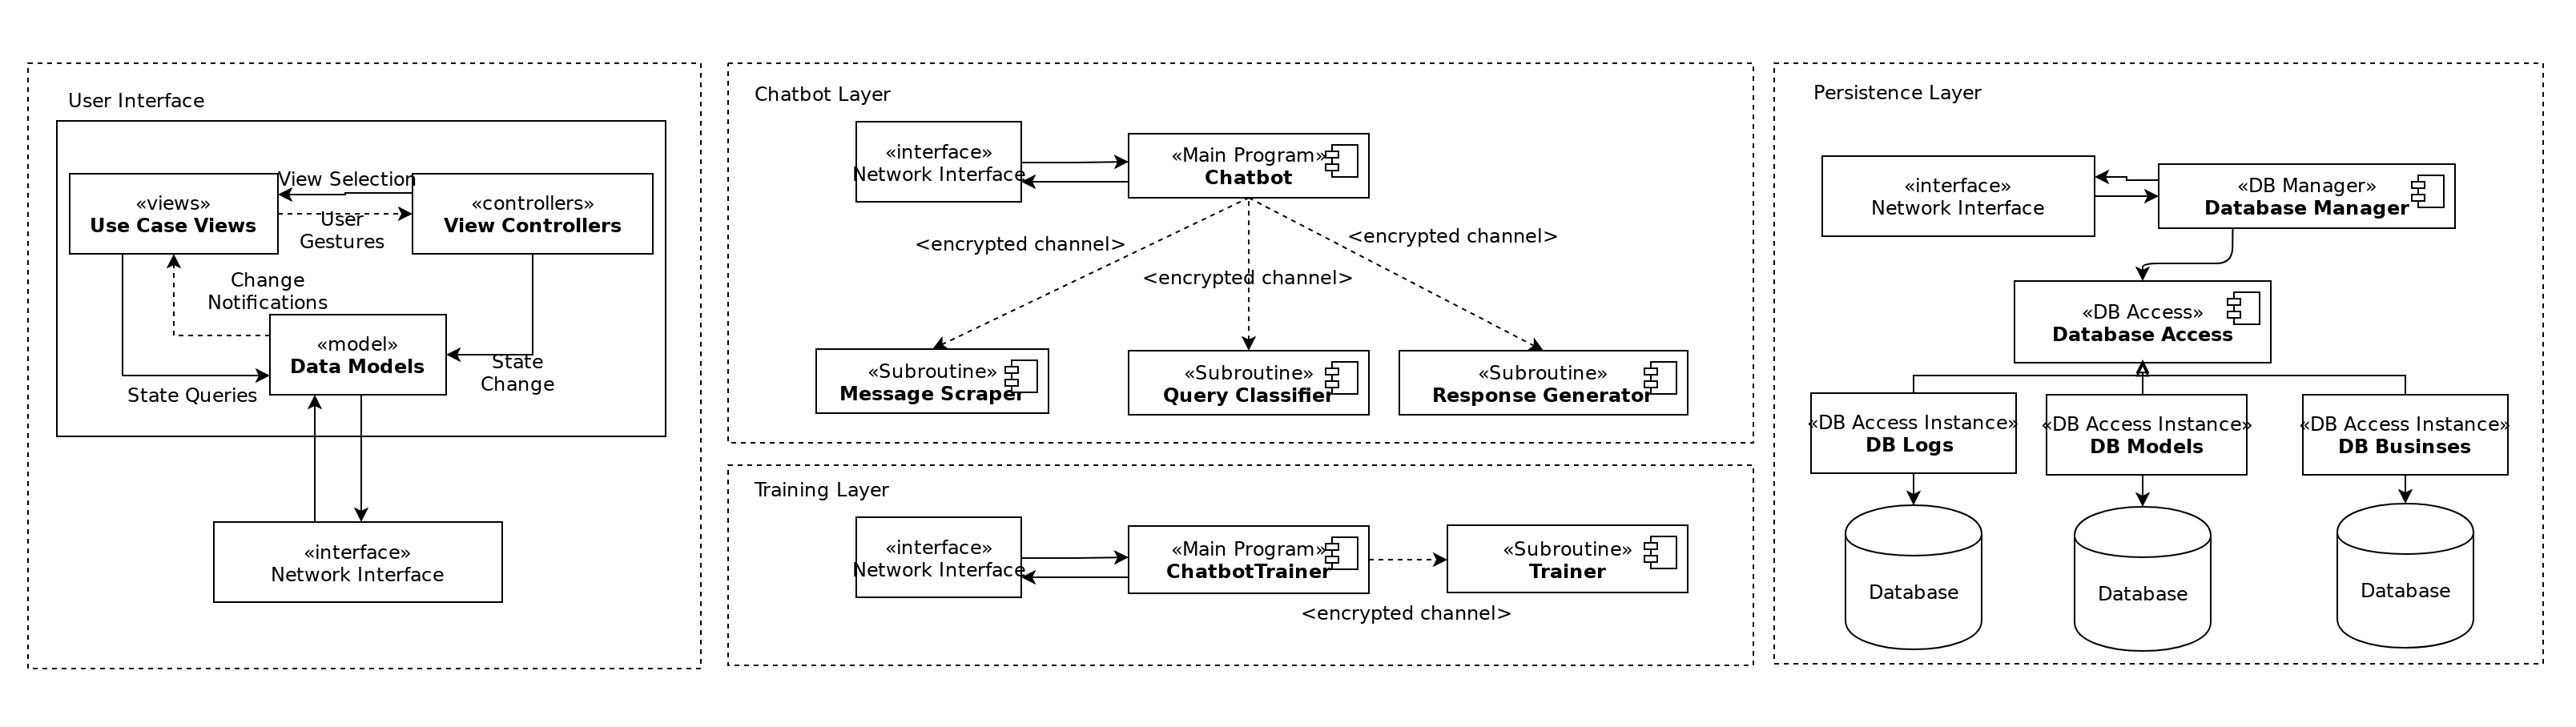
\includegraphics[width=1.25\textwidth]{../../images/Botic_Layered_Architecture.png}
	\caption{Architectural Stye of the System}
\end{figure}

The allowed-to-use relation here is denoted by the geometric adjacency of the layers from left to right-- layers on the left use layers on the right and the layers on the right are used by the layers on the left. The exception here is the connection between the user interface as well as the persistence layer, as this is required to store information from controllers within the UI's MVC architecture, as well as obtaining information or data for UI level use case i.e. displaying users or obtaining user information. The connections between each layer are made to be through encrypted channels. An appropriate technology will be used to implement this during the implementation phase e.g. SSL.

\subsubsection{The User Interface Subsystem}
The User Interface Layer that is also an interactive subsystem uses an MVC architectural style. Using this architectural style, we ensure that user interface interface functionality, something that tends to change frequently especially in response to knew design trends *Quote IMY theory notes, be kept seperate from the application functionality and yet be ever responsive to user input, the most important thing in an interactive system\cite{Book:2}. This is the solution:

\begin{figure}[H]
	\centering
	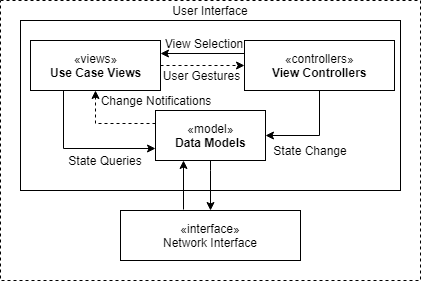
\includegraphics[width=0.5\textwidth]{../../images/User_Interface_MVC.png}
	\caption{Architectural Style of the User Interface}
\end{figure}

\subsubsection{The Chatbot Layer}
The Chatbot Layer is a transformational subsystem, and will use a Main Program and Subroutines architectural style.

\begin{figure}[H]
	\centering
	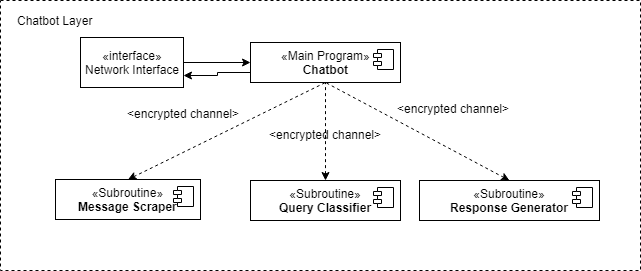
\includegraphics[width=0.8\textwidth]{../../images/Chatbot_Layer_Architecture.png}
	\caption{Architectural Style of the Chatbot Layer}
\end{figure}

\subsubsection{The Training Layer}
This layer is a transformational subsystem and will also use a Main Program and Subroutines architectural style.

\begin{figure}[H]
	\centering
	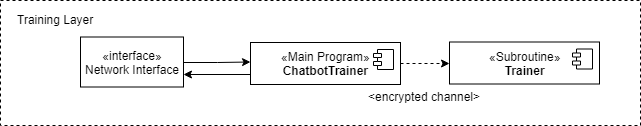
\includegraphics[width=0.8\textwidth]{../../images/Training_Layer_Architecture.png}
	\caption{Architectural Style of the Training Layer}
\end{figure}

The ChatbotTrainer is a single container that has 4 instances: these are to service requests from the user interface (requests which are sent by the Administrator user), one to train the Message Scraper, one to train the Classifier, and one to train the Response Generator. It uses the Strategy Desgin Pattern to switch different training strategies/methods to suit each subsystem it services. This results in multiple instances of the same subsystem, but each using a different training method and data on a different chatbot subsystem.

\subsubsection{The Persisitance Layer}
This layer is a clear candidate for the Persistence Framework architectural style, and it's architectural style is just that. Here is our solution:

\begin{figure}[H]
	\centering
	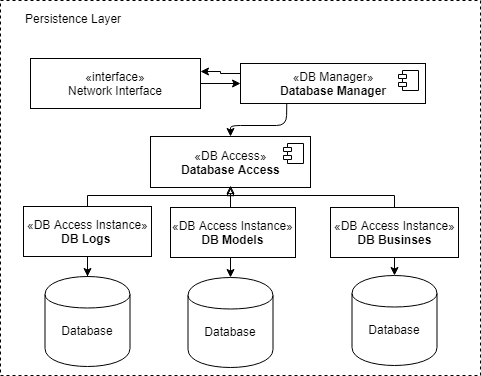
\includegraphics[width=0.6\textwidth]{../../images/Persistence_Layer_Architecture.png}
	\caption{Architectural Style of the Persistence Layer}
\end{figure}

In accordance to the architectural tactics we have chosen to observe to achieve availability and security quality attributes and requirements, in particular the security tactic to seperate access and data of different sensitivities, we have made the decision to have three databases. The first is for logs and audit trails, the second for the data models what would be used for the chatbot subsystems, and the third for recording queries and responses-- data that is concerned with the functional business processes.

\section{References}
\bibliographystyle{IEEEtran}
\bibliography{references}
%%IEEE. IEEE Std 830-1998 IEEE Recommended Practice for Software Requirements Specifications. IEEE Computer Society, 1998
%%http://www.cse.msu.edu/~chengb/RE-491/Papers/SRSExample-webapp.doc
%%TripleParity docs

\end{document}